% tbsrc/grid.tex — The Image: Voxel Grid and Conventions
% Status: written (first draft). Voxel grid + voxelization figure, the two roles
% of voxsize, choosing the voxel size, FOV. Julia specifics are in footnotes.
\section{The Image: Voxel Grid and Conventions}
\label{sec:grid}

The activity image is the unknown of the reconstruction. This section fixes how
the continuous field $f$ of Section~\ref{sec:intro:problem} is represented on a
grid, the conventions that tie that grid to the same world frame as the LOR
endpoints, and how the grid spacing relates to the resolution the image can
represent.

\subsection{The voxel grid}
\label{sec:grid:grid}

The image is a three-dimensional array of $\bm{n}=(n_0,n_1,n_2)$ voxels, read as
the non-negative vector $\xv\in\RR^N_{\ge0}$ with $N=n_0 n_1 n_2$. The grid is
fixed by three things: its shape $\bm{n}$, the voxel size
$\bm{\Delta}=(\Delta_0,\Delta_1,\Delta_2)$ in millimetres, and an origin
$\bm{o}$, the world coordinate of the centre of the first
voxel.\footnote{In Julia this origin is the \code{img\_origin} argument and the
centre of \code{img[1,1,1]} (1-based indexing); the projector kernels, inherited
from the C reference, label the same corner voxel $(0,0,0)$ --- a labelling
difference only. A grid centred on the world origin is obtained with
\code{org = -(n .- 1) .* voxsize ./ 2}, i.e.\ Eq.~\eqref{eq:grid-center}.}
The centre of voxel $(j_0,j_1,j_2)$ is then
\begin{equation}
  \bm{u}_{\bm j} = \bm{o}
    + \bigl((j_0-1)\Delta_0,\,(j_1-1)\Delta_1,\,(j_2-1)\Delta_2\bigr),
  \qquad j_k = 1,\dots,n_k ,
  \label{eq:grid-map}
\end{equation}
and between voxel centres $f$ is reconstructed by trilinear interpolation, as the
projector requires (Section~\ref{sec:projection:lineintegral}).
Figure~\ref{fig:grid-voxelization} shows the result: a continuous activity field
and its representation on the grid. To centre the grid on the world origin ---
the usual choice, with the scanner axis through the middle --- set
\begin{equation}
  \bm{o} = -\tfrac12(\bm{n}-\bm{1})\odot\bm{\Delta} .
  \label{eq:grid-center}
\end{equation}
The origin, the voxel sizes, and the LOR endpoints all live in one millimetre
frame (Section~\ref{sec:geometry:endpoint}); keeping them consistent is
essential, and the single most common source of error.

\begin{figure}[t]
  \centering
  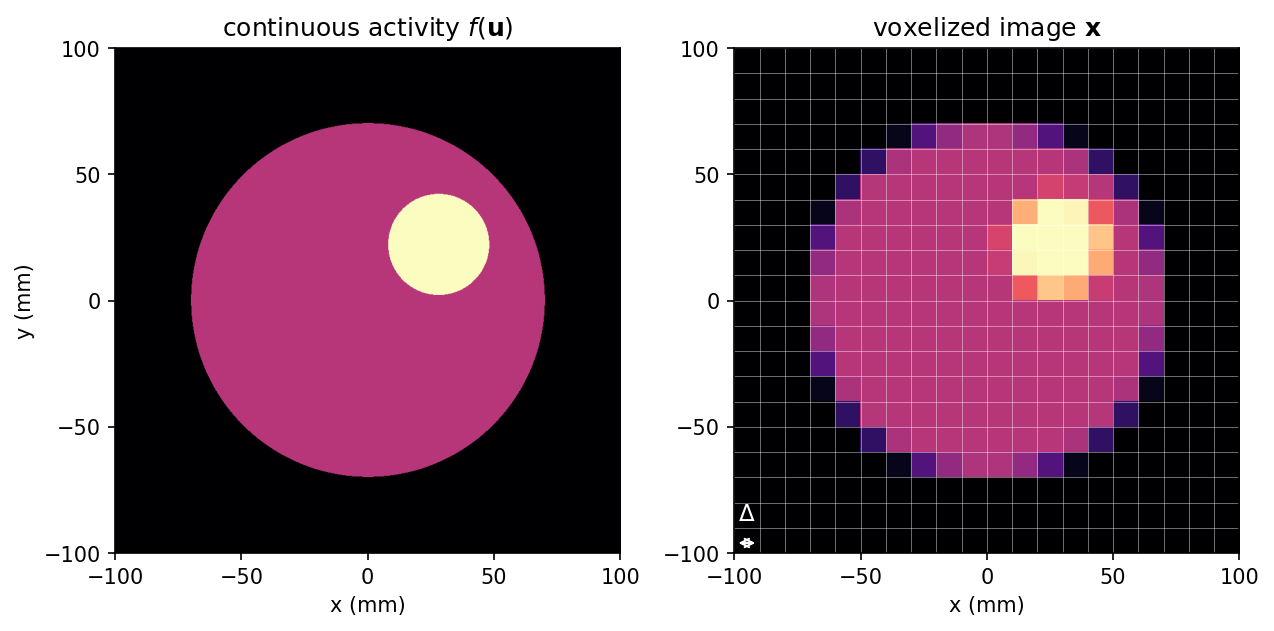
\includegraphics[width=0.92\textwidth]{figures/voxelization.png}
  \caption{Voxelization of the image. A continuous transverse activity
    distribution $f(\bm{u})$ (left) is represented on a voxel grid of spacing
    $\bm{\Delta}$ (right): each voxel carries a single value of $\xv$, and $f$ is
    recovered between voxel centres by trilinear interpolation. The grid is
    deliberately coarse here to make the voxels visible.}
  \label{fig:grid-voxelization}
\end{figure}

\subsection{Two roles of the voxel size}
\label{sec:grid:voxsize}

$\bm{\Delta}$ does double duty, and both matter. It \emph{places} the grid in
the world through \eqref{eq:grid-map}, converting voxel indices to millimetres
and back --- this is what lets a ray be intersected with the image box. And it
\emph{scales the line integral}: Joseph's method sums interpolated values over
voxel planes and multiplies by the path-length correction
$c=\Delta_{\mathrm{dir}}/\abs{\cos\theta_{\mathrm{dir}}}$
(Section~\ref{sec:projection:joseph}), with $\Delta_{\mathrm{dir}}$ the voxel
size along the ray's principal axis. A wrong voxel size therefore corrupts both
the geometry and the quantitative scale of the projection.

\subsection{Choosing the voxel size}
\label{sec:grid:resolution}

The voxel size controls how finely the image samples space; the spatial
resolution it can represent is set separately, by the detector and the data
(Section~\ref{sec:resolution}). The grid should be fine enough to sample that
resolution, which fixes a useful rule of thumb:
\begin{equation}
  \Delta \;\approx\; \tfrac13\ \text{to}\ \tfrac12\ \text{of the resolution }\FWHM .
  \label{eq:grid-sampling}
\end{equation}
At this spacing the grid captures the resolution the scanner delivers;
substantially coarser blurs it further, while much finer only inflates $N$ ---
and the reconstruction cost and the noise per voxel --- with no gain in detail.
The voxels need not be cubic: anisotropic $\bm{\Delta}$ is allowed, and is
natural when the axial sampling differs from the transverse. For a
$3.5\,\mathrm{mm}$-FWHM scanner such as CRYSP, \eqref{eq:grid-sampling} points to
roughly $1.2$--$1.8\,\mathrm{mm}$ voxels.

\subsection{Field of view}
\label{sec:grid:fov}

The grid should cover the region the scanner can image. Transversely the field
of view is bounded by the bore radius (which limits where LORs cross); axially it
is the ring span, or the axial field of view of a continuous scanner
(Section~\ref{sec:geometry}). Voxels well outside the measured LORs are crossed
by no ray: they accrue no sensitivity, and the reconstruction leaves them
untouched (Section~\ref{sec:mlem}). Sizing $\bm{n}\odot\bm{\Delta}$ to the field
of view, with the centred origin \eqref{eq:grid-center}, is the standard setup
the examples use.
